\documentclass[a4paper,12pt]{article}
	\usepackage[ansinew]{inputenc}
	\usepackage{ae}
	\usepackage[brazil]{babel}
	\usepackage{xcolor}
	\usepackage{graphicx} % <-- Permite inserir figuras.
	
	\newcommand{\comando}[1]{{\textbackslash\textcolor{blue}{#1}}}
	\newcommand{\ambiente}[1]{{\textcolor{green}{#1}}}
\begin{document}
		
	\noindent\hrulefill
	\begin{minipage}[c]{0.5\textwidth}
		\setlength{\parindent}{1em}
	
		\tiny
		Tanto o comando \comando{parbox} como o ambiente \ambiente{minipage} criam uma caixa ao redor de textos longos (ou figuras, tabelas, etc). A diferença é que o primeiro não pode ser aplicado para mais de um parágrafo, enquanto	o \ambiente{minipage} pode.
		
		Além disso, a sintaxe do \ambiente{minipage} é mais inteligível que a do \comando{parbox}. Isto o torna particularmente recomendável quando o conteúdo que se quer colocar numa caixa é extenso. Por conseguinte, o \comando{parbox} costuma ficar destinado a caixas menores.
		
		Outra diferença importante é que dentro do escopo da mini-página o comprimento \comando{textwidth} é igual à largura da própria mini-página, o argumento obrigatório do ambiente \ambiente{minipage}.
	\end{minipage}%
	\hrulefill
	\fbox{%
	\begin{minipage}[c]{0.3\textwidth}
		% O comando \includegraphics, do pacote graphicx, permite inserir figuras no seu arquivo LaTeX. Mas veremos isto depois.
		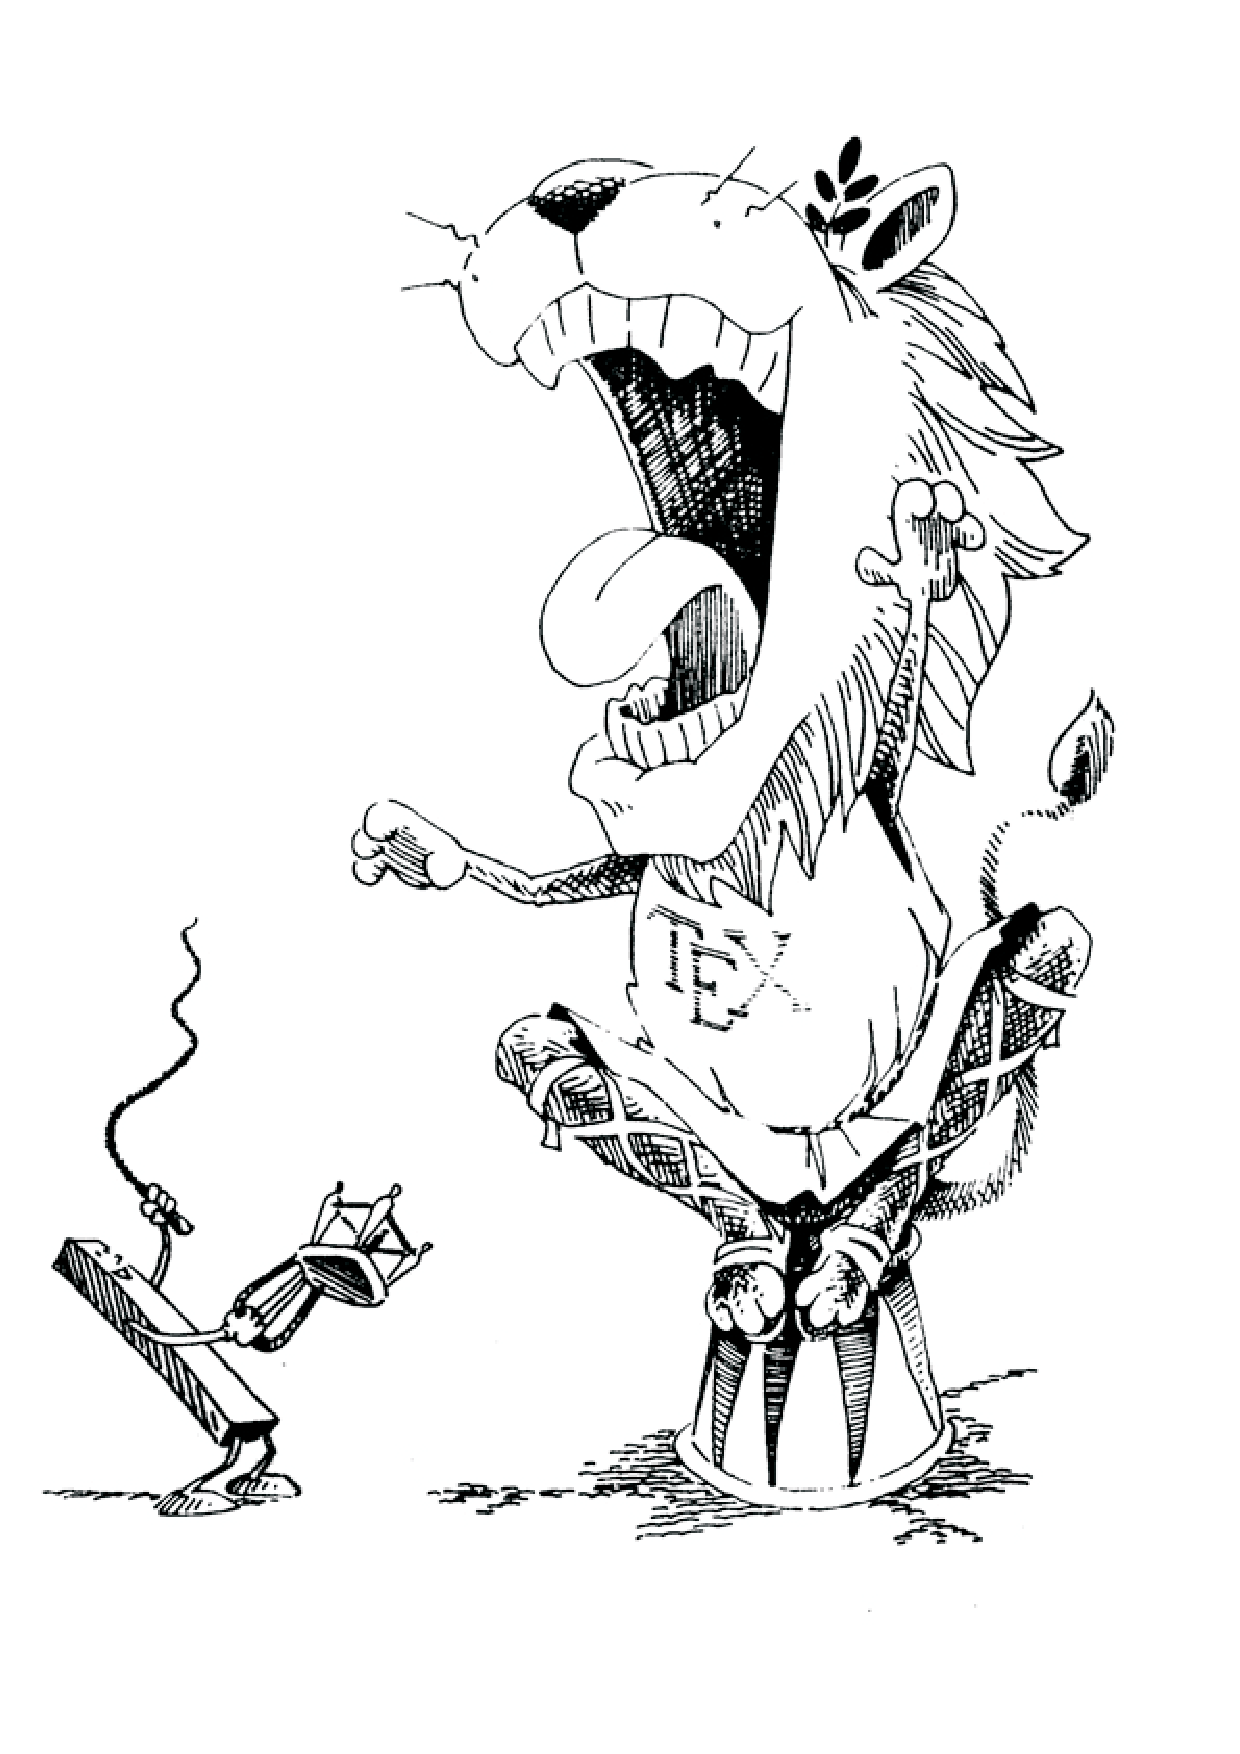
\includegraphics[width=\textwidth]{controlling_TeX}
	\end{minipage}}%
	\hrulefill
	
	% Experimente mudar o parâmetro opcional de \parbox de ambas as caixas. Você pode usar t (de top: topo), c (de center: centro) ou b (de bottom: abaixo).

\end{document}